\documentclass[convert]{standalone}

\usepackage{tikz}
\usepackage{graphicx}
\pagestyle{empty}

% INT_AY22_L11_Fig04_Vector_diagrams.png

\begin{document}
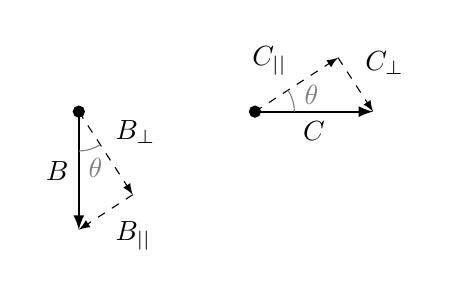
\begin{tikzpicture}[> = latex]

% Define the ramp angle

\def\Q{33}
	
\matrix[column sep = 1 cm]{
	
	% The dot
	
	\filldraw (0, 0) circle (2 pt);
	
	% Vector B
	
	\draw [->, thick] (0, 0) -- node [left] {$B$} (270 : 1.5);
	
	% Vector components
	
	\draw [dashed, ->] (0, 0) -- node [above right] {$B_\perp$} (270 + \Q : {1.5 * cos(\Q)}) coordinate (B-perp);
	\draw [dashed, ->] (B-perp) -- node [below right] {$B_{||}$} ++ (180 + \Q : {1.5 * sin(\Q)});
	
	% Angle indicator
	
	\draw [gray] (0, -0.5) arc (270 : 270 + \Q: 0.5);
	\node [gray] at ({270 + 0.5 * \Q} : 0.75) {$\theta$};

&
	
	% The dot
	
	\filldraw (0, 0) circle (2 pt);
	
	% Vector C
	
	\draw [->, thick] (0, 0) -- node [below] {$C$} (0 : 1.5);
	
	% Vector components
	
	\draw [dashed, ->] (0, 0) -- node [above left] {$C_{||}$} (\Q : {1.5 * cos(\Q)}) coordinate (C-par);
	\draw [dashed, ->] (C-par) -- node [above right] {$C_\perp$} ++ (270 + \Q : {1.5 * sin(\Q)});
	
	% Angle indicator
	
	\draw [gray] (0.5, 0) arc (0 : \Q: 0.5);
	\node [gray] at ({0.5 * \Q} : 0.75) {$\theta$};

\\
};		
\end{tikzpicture}
\end{document}